%%
%% This is file `example-1.tex',
%% generated with the docstrip utility.
%%
%% The original source files were:
%%
%% drexel-thesis.dtx  (with options: `example-part')
%% 
%% This is a generated file.
%% 
%% Copyright (C) 2010 W. Trevor King
%% 
%% This file may be distributed and/or modified under the conditions of
%% the LaTeX Project Public License, either version 1.3 of this license
%% or (at your option) any later version.  The latest version of this
%% license is in:
%% 
%%    http://www.latex-project.org/lppl.txt
%% 
%% and version 1.3 or later is part of all distributions of LaTeX version
%% 2003/06/01 or later.
%% 

\chapter{Population activity encoding }

Individual neurons in the brain are tuned to fire upon specific events such as visual stimuli of a particular type \citep{Hubel1962} .
However, even neurons that are tuned to a specific stimulus show variability in their firing rate and timing when the same stimulus is repeatedly applied \citep{Georgopoulos1982}\citep{Newsome1989}.
This indicates that individual neurons do not reliably encode sensory information, and therefore information in the brain must be represented by the firing dynamics of populations of many neurons.
This neuron population coding may take the form of variations in the average firing rate of the neurons in the population (rate coding) or variations in the synchronization between neuron spikes (temporal coding).
The temporal and rate coding may also have a functional relation, i.e. through Hebbian learning \citep{Basawaraj2019}.
Various methods of decoding the information in these population dynamics have been studied \citep{Deneve1999}\citep{Xu2019}, 
and population dynamics are incorporated into modern theories of neural computation \citep{Pitkow2017}\citep{Nadeau2020}.

Here we consider how information that is represented as population activity in one cortical area could be transferred to another cortical area via traveling waves.
For example, \citet{Heitmann2013} proposed a possible mechanism for decoding traveling waves and provided applications to the motor cortex.
Direct connections between spatially separated cortical areas are quite sparse\citep{Markov2011} as intra-cortical connectivity is mostly local in nature.
Traveling waves of neuronal activity would provide a mechanism for long-range information transfer across cortical areas 
even if there were very few direct neural connections between those areas.

To test our hypothesis of information coding and transfer we first define a population of input neurons.
These input neurons represent a neural population that is e.g. tuned to the same orientation of visual stimulus, 
so that the stimulus or other information is encoded in the firing rate of this population.
We represent the information as an average firing rate.
We simulate the population of input neurons as independent Poisson processes with the common average firing rate.
We then perform simulations of neural system to determine if the information, encoded in the firing rate of the input population,
can be transferred via traveling waves.

We have previously shown that our minicolumn model supports stimulus-evoked traveling waves across a variety of model parameters.
We expect most activity in the minicolumn to result from distinct traveling waves, so it is natural to characterize the traveling waves as atomic units of information.
The number of waves per second that travel through the minicolumn, which we term the wave arrival rate, increases as the average firing rate of the input pool of neurons is increased.
The wave arrival rate increases asymptotically with the input population firing rate in a manner that resembles the activation functions of either a single neuron or a population of neurons.
This leads us to consider the minicolumn to possess a nonlinear activation function of input population firing rate, 
and to consider the minicolumn as encoding the input population firing rate into the wave arrival rate.

\section{Population activity representation}
To understand how our minicolumn may encode and transmit information that is represented as the activity of a population of neurons.
Individual neurons in the cortex fire irregularly \citep{Maimon2009}, and the spike timing of a single neuron is generally characterized by a Poisson process with some average firing rate \citep{Gerstein1964}.
The external stimulus $I_i^{stim}$ in our simulations is generated from a population of 50 neurons that emit spikes according to independent Poisson processes characterized by a common firing rate.
Each neuron $j$ in the input population of Poisson neurons is connected to each neuron $i$ in the bottom layer (all minicolumn neurons with Z=0) of the minicolumn with probability $P_{ij} = 1/2$.
The stimulus applied to the bottom layer is given by:
\begin{align}
 \begin{split}
  I_i(t)^{stim} &= \sum_{i,j} \sum_{t^\prime_j} S_{ij}  \Theta(t-t^\prime_j)e^{-(\frac{t-t^\prime_j}{\sigma_e})^2}\\
  S_{ij}^{excitatory} &= K^{stim} \times \mathcal{U}\{0,0.5 \} \text{ if i,j connected}\\
  S_{ij}^{inhibitory} &= K^{stim} \times \mathcal{U}\{-1,0 \} \text{ if i,j connected}\\
  S_{ij} &= 0 \text{ if i,j not connected}
 \end{split}
\end{align}
where $t^\prime_j$ are the spike times of Poisson neuron $j$, $\sigma_e=2\ ms$ is a synaptic response time constant as described above, and $K^{stim}$ is an overall connection strength weight as described above.


\section{Traveling wave encoding}
Our first configuration is an minicolumn consisting of four minicolumns, each with dimensions $2x2x40$ (X/Y/Z).
The minicolumn parameters are $C=0.5$, $\lambda=2.5$, $\kappa=0.1$, $K^{minicolumn}=24$ and $K^{stim}=6$.
The other parameters are fixed for all experiments as described in Methods.

We stimulated the minicolumn using several instantaneous firing rates for the input population.
Traveling waves are evoked in the minicolumn for higher firing rates (Figure \ref{fig:sce_raster}).

\begin{figure}[!htb]
 \centering
 \caption{Poisson spike trains in the input population (bottom) evoke traveling waves in the minicolumn (top). 
	  Raster plots are shown for firing rates of 1 spike/second (left), 5 spikes/second (middle) and 21 spikes/second (right).  }
 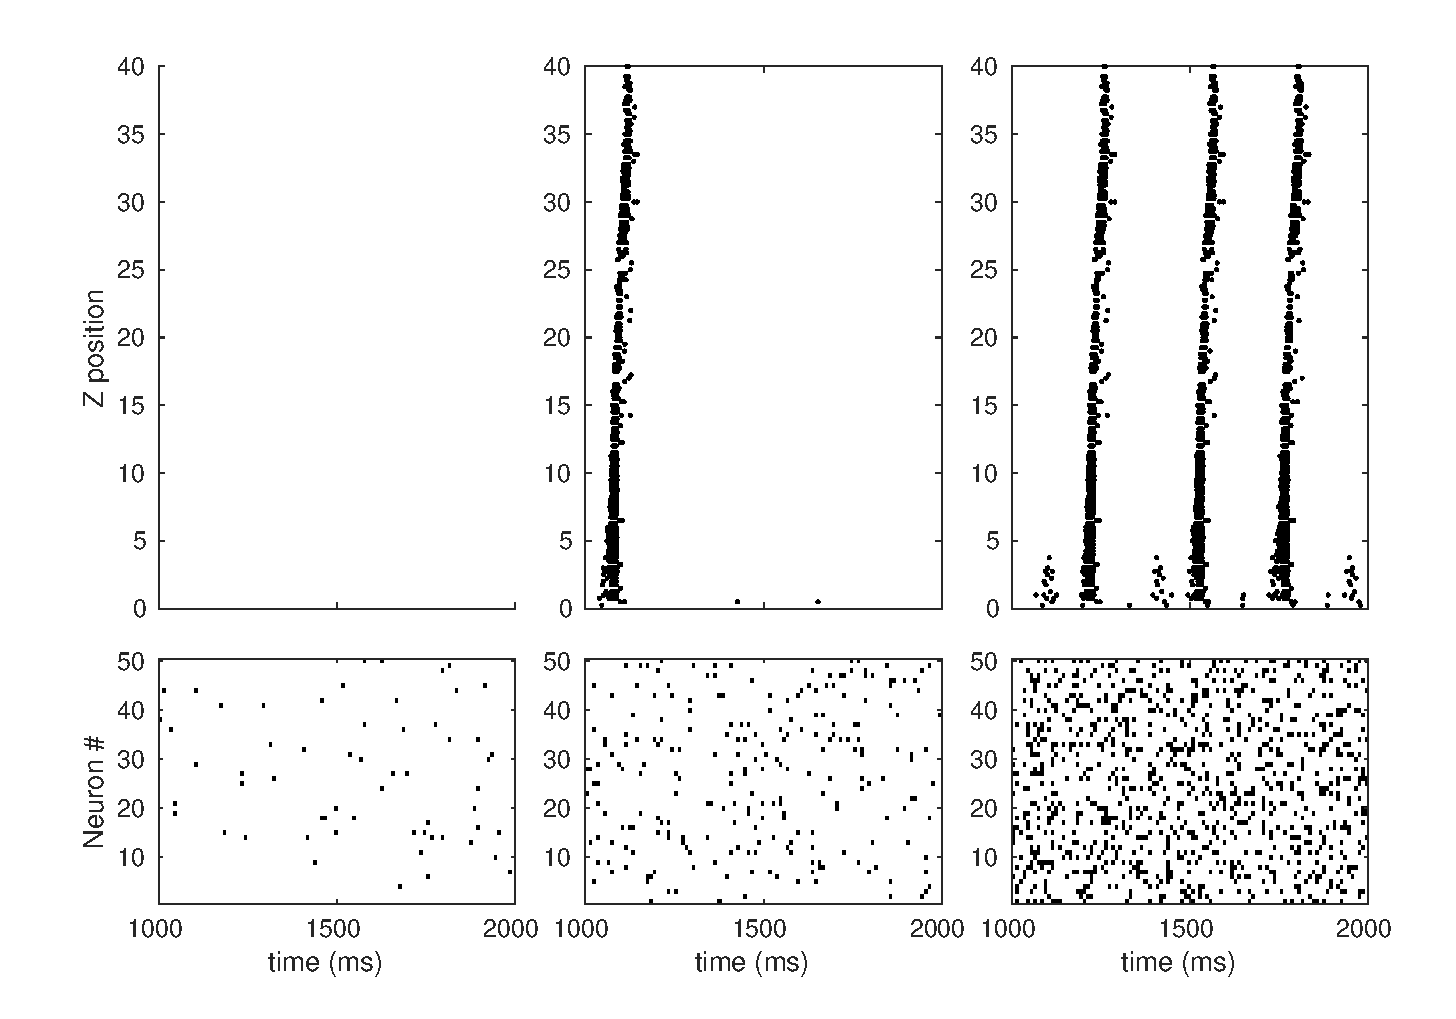
\includegraphics[width=\textwidth]{fig/SCE_2x2_FRE_rasters}
 \label{fig:sce_raster}
\end{figure}

\FloatBarrier

We stimulated the minicolumn with instantaneous firing rates from 1 to 21 spikes/second, with 100 random inputs created for each firing rate.
The resulting waves rates are shown in Figure \ref{fig:sce_activation_function}.
The mean wave rate showed a clear trend that is similar to a logarithmic curve. 
It also resembled the population activation rate shown in \citet{Trappenberg2010} Eq. 3.43 for the response of a population of neurons to slowly varying inputs:
\begin{align}
 g(x) &= \frac{1}{t^{ref}-\tau \log{(1-\frac{1}{\tau x})}}
\end{align}
where $t^{ref}$ is an absolute refractory period and $\tau$ is the characteristic response time.
We therefore consider our minicolumn to have an nonlinear activation function when stimulated by a  population of neurons.
This demonstrated that the minicolumn can be said to encode the population rate into the wave rate in a analogous manner to which single neurons and populations of neurons 
encode their stimulus strength into their firing rate.

\begin{figure}[!htb]
 \centering
 \caption{The minicolumn encodes the input population firing rate into the wave arrival rate. 
          Wave arrival rates are measured across 100 trials of randomly generated spike trains for each input firing rate.
          Error bars are $\pm \sigma$. }
 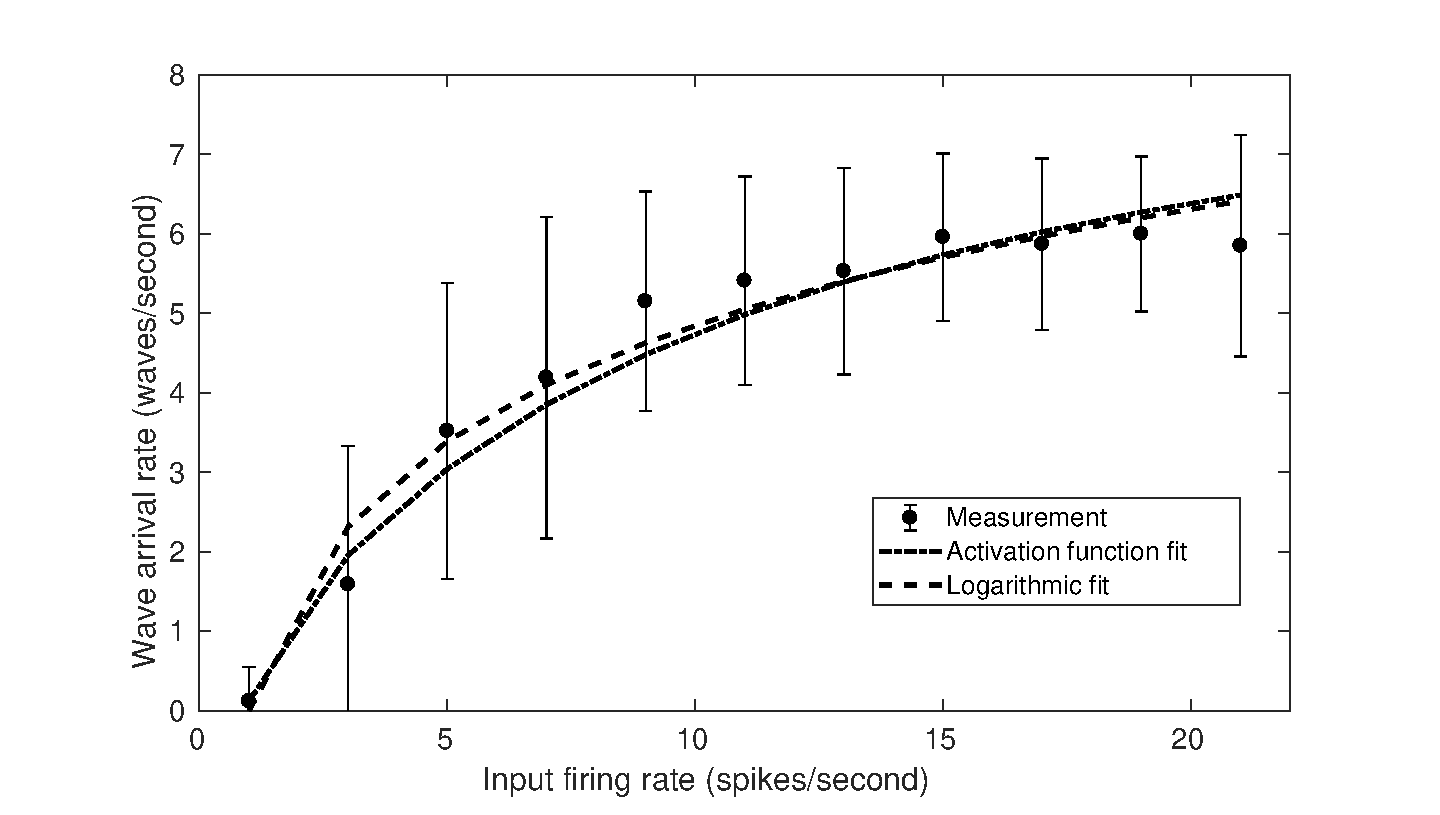
\includegraphics[width=\textwidth]{fig/SCE_2x2_FRE}
 \label{fig:sce_activation_function}
\end{figure}

Although the mean wave rates showed a clear trend, the trial-to-trial wave rates were highly variable. 
This indicates that our single minicolumn would not reliably encode population rate into wave rate.

\FloatBarrier

Like our minicolumn, individual neurons also have variable firing responses to identical stimuli.
This variability is one of the key motivations for the population activity theories of information encoding in the cortex.
We next followed a similar approach and investigated the activation function of a population of multiple redundant minicolumns.
This is similar to our forest of minicolumns, except the overall system is still much longer in the Z dimension than the X and Y dimension.

We first evaluated a forest with a side spacing of $4\lambda$ between the minicolumns.
At this wide spacing the four minicolumns are almost completely disconnected.
The results are shown in Figure \ref{fig:forest_encoding_separate}.
With multiple independent minicolumns the total wave arrival rates were higher since each minicolumn supported independent waves.
The trials of different stimulus generated for the same average firing rate still show substantial variability.
\begin{figure}[!htb]
 \centering
 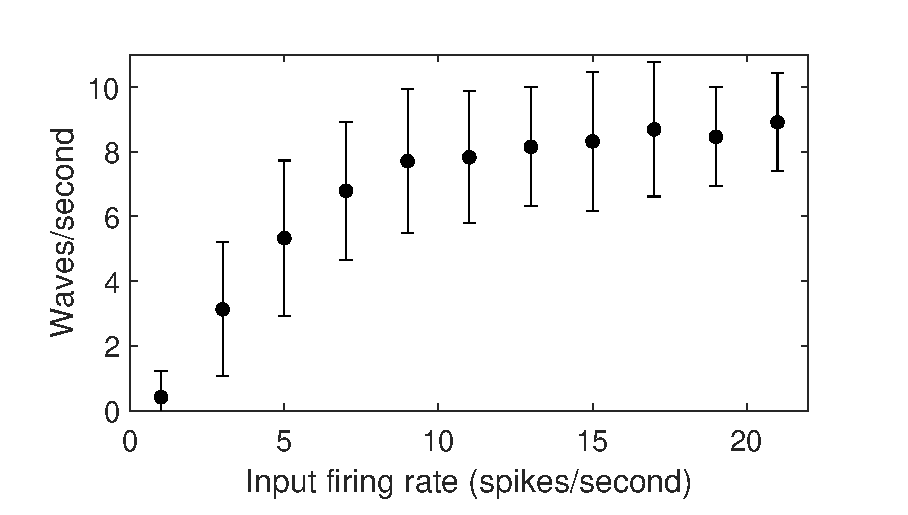
\includegraphics[width=0.6\textwidth]{fig/ForestEncoding_FourLambda}
 \caption{Firing rate-to-wave rate activation function of a forest of 4 minicolumns separated by $4\lambda$.
          Each minicolumn is 2x2x40.
          100 trials were performed for each value of the input firing rate, error bars are $\pm \sigma$.
          The encoding of the input population firing rate into the wave rate was still highly variable.}
 \label{fig:forest_encoding_separate}
\end{figure}
\FloatBarrier

We then repeated the simulation using a forest of minicolumns separated by $1\lambda$ (Figure \ref{fig:forest_encoding_coupled}).
The coupled minicolumns show a more consistent activation function with lower variability.

\begin{figure}[!htb]
 \centering
 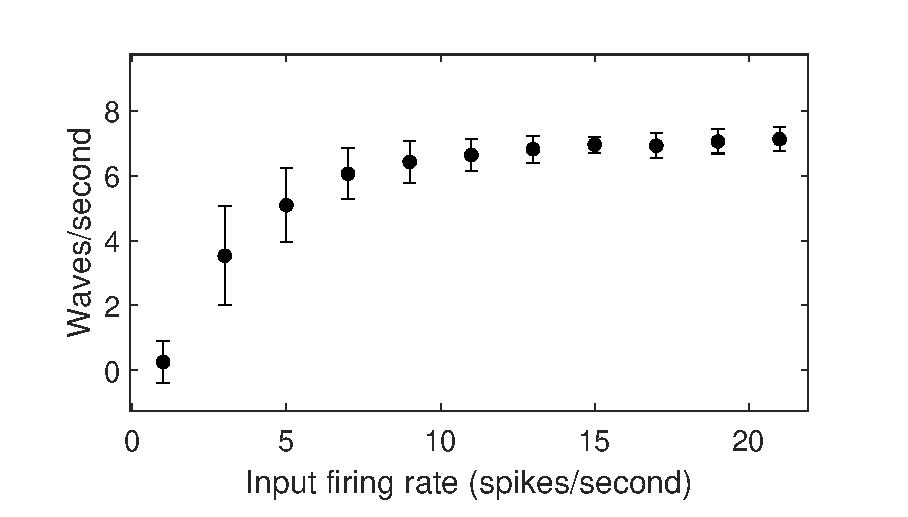
\includegraphics[width=0.6\textwidth]{fig/ForestEncoding_OneLambda}
 \caption{Firing rate-to-wave rate activation function of a forest of 4 minicolumns separated by $1\lambda$.
          Each minicolumn is 2x2x40.
          100 trials were performed for each value of the input firing rate, error bars are $\pm \sigma$.
          The encoding of the input population firing rate into the wave rate was much less variable.}
 \label{fig:forest_encoding_coupled}
\end{figure}
\FloatBarrier


\endinput
%%
%% End of file `example-1.tex'.
